% Created 2017-05-29 lun. 17:35
\documentclass[smaller]{beamer}
\usepackage[utf8]{inputenc}
\usepackage[T1]{fontenc}
\usepackage{fixltx2e}
\usepackage{graphicx}
\usepackage{grffile}
\usepackage{longtable}
\usepackage{wrapfig}
\usepackage{rotating}
\usepackage[normalem]{ulem}
\usepackage{amsmath}
\usepackage{textcomp}
\usepackage{amssymb}
\usepackage{capt-of}
\usepackage{hyperref}
\usepackage[T1]{fontenc}
\usepackage[english, frenchb]{babel}
\useoutertheme{infolines}
\mode<beamer>{\usetheme{Pittsburgh}}
\setbeamertemplate{navigation symbols}{}
\setbeamerfont{structure}{series=\bfseries}
\setbeamertemplate{items}[triangle]
\setbeamercolor{block title}{fg=blue!40!black}
\newcommand{\shorttitle}{OTB User Days, June 7-9 2017}
\newcommand{\shortauthor}{}
\setbeamertemplate{footline}{\leavevmode\hbox{\begin{beamercolorbox}[wd=.333333\paperwidth,ht=2.25ex,dp=1ex,left]{author in head/foot}  \usebeamerfont{author in headfoot}\insertshortinstitute~~\shortauthor   \end{beamercolorbox}   \begin{beamercolorbox}[wd=.333333\paperwidth,ht=2.25ex,dp=1ex,center]{title   in head/foot}     \usebeamerfont{title in head/foot}\shorttitle   \end{beamercolorbox}   \begin{beamercolorbox}[wd=.333333\paperwidth,ht=2.25ex,dp=1ex,right]{date in head/foot}\usebeamerfont{date in head/foot}\insertshortdate{} \hspace*{2em}\insertframenumber{} / \inserttotalframenumber\hspace*{2ex} \end{beamercolorbox}}\vskip0pt}
\institute{ 
\includegraphics[width=0.6cm]{images/logoIncrust.png}}
\usepackage{fourier}
\usepackage{amsfonts,bm,amsmath,amssymb,ifsym,marvosym,tabularx,array,ifsym}
\usepackage{tikz}
\usetikzlibrary{arrows,fit,backgrounds,positioning,shapes,shadows}
\newcommand{\vns}{Ven$\mu$s}
\newcommand\boxPlot[6] {  \pgfmathsetmacro\rectSize{0.3};  \draw[thick] (#2,#1) -- (#3,#1);  \draw[thick] (#2,#1-\rectSize/2) -- (#2,#1+\rectSize/2);  \draw[thick] (#5,#1) -- (#6,#1);  \draw[thick] (#6,#1-\rectSize/2) -- (#6,#1+\rectSize/2);  \draw[fill=white] (#3,#1-\rectSize) rectangle (#5,#1+\rectSize);  \draw (#4,#1-\rectSize) -- (#4,#1+\rectSize);}
\def\G{\ensuremath{{\cal G}}}
\newcommand{\putat}[3]{\begin{picture}(0,0)(0,0)\put(#1,#2){#3}\end{picture}}
\pgfdeclareimage[height=96mm,width=130mm]{background}{images/fondsClairSansLogo}
\setbeamertemplate{background}{\pgfuseimage{background}}
\subtitle{Introduction}
\usetheme{default}
\author{OTB Team}
\date{05/06/2017}
\title{OTB Users Days 2017}
\hypersetup{
 pdfauthor={OTB Team},
 pdftitle={OTB Users Days 2017},
 pdfkeywords={otb},
 pdfsubject={},
 pdfcreator={Emacs 24.5.1 (Org mode 8.3.3)}, 
 pdflang={Frenchb}}
\begin{document}

\maketitle

\section{Introduction}
\label{sec:orgheadline9}
\begin{frame}[label={sec:orgheadline1}]{Welcome to OTB Users Days 2017!}
\begin{center}
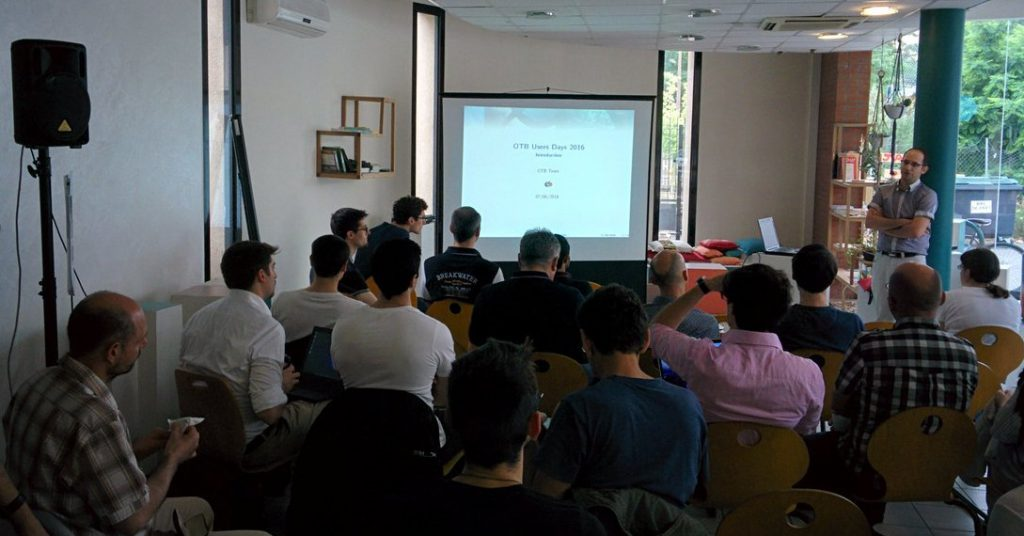
\includegraphics[width=0.8\textwidth]{images/img1-1024x536.jpg}

PSC meeting during OTB Users Days 2016 (second edition)
\end{center}
\end{frame}

\begin{frame}[label={sec:orgheadline2}]{Recap of OTB Users Days 2015}
\begin{block}{Day 1}
\begin{itemize}
\item Presentations from the OTB development team at CNES and CS :
Introduction, What’s new in OTB? open governance, Monteverdi\ldots{} for OTB: thoughts and context

\item Users

\begin{itemize}
\item Big Data Solutions for EO pursued at JRC – P. Kempeneers \& D. De Marchi (JRC)

\item OTB for BIOMASS – T. Koleck (CNES)

\item Using OTB for processing UAS imagery – A. Lobo (CSIC)

\item Geosigweb – C. Bisso (Geosigweb)
\end{itemize}

\item Then Tech talks:

\begin{itemize}
\item How we plan to do MPI-powered OTB (see rfc-26)

\item The new flexible classification framework in OTB

\item Machine learning in OTB: s/opencv/shark/

\item S1 Geometry in OTB
\end{itemize}
\end{itemize}
\end{block}
\end{frame}

\begin{frame}[label={sec:orgheadline3}]{Recap  Day 2}
\begin{block}{Tutorials}
Introduction to Monteverdi 3.0
OTB tools for image segmentation
Discover the new applications (Classification, Polarimetry)
The steganography game
Reminder about applications framework and extended filenames
Write your own remote module
\end{block}
\begin{block}{Brainstorming}
\end{block}
\end{frame}

\begin{frame}[label={sec:orgheadline4}]{Recap day 3}
\end{frame}

\begin{frame}[label={sec:orgheadline5}]{This year: program 2017}
\url{https://huit.re/otb_users_days_2017}
\end{frame}
\begin{frame}[label={sec:orgheadline6}]{Day 1: Talks}
\begin{itemize}
\item 15/20 min talks and leave 5/10 minutes for questions
\item Language for the event will most probably be French
\item However slides and materials should be in English if possible
\item In parallele: organize Day 2 and 3 (check with session leaders)
\end{itemize}
\end{frame}
\begin{frame}[label={sec:orgheadline7}]{Day 2: Parallel sessions}
\begin{itemize}
\item Tutorials
\item Open question \& features requests \& one-on-one tutoring
\item Brainstorming
\end{itemize}
\end{frame}
\begin{frame}[label={sec:orgheadline8}]{Day 3: Hackfest}
\begin{itemize}
\item Keynote talks: C++11 for OTB?
\item Then 30 minutes planning meeting at the beginning
\item Write the code you need with the help of a member of the
development team
\item Documentation review: live enhancement of the documentation
\item Live bugfixes: You think you found a bug? We investigate and fix it with you
\item Packaging improvement
\item PSC meeting (to be scheduled)
\item If there is time left: guru code hacking
\end{itemize}

\alert{Lunch: Pizza party!}

\begin{block}{This is not a 1000+ participants IEEE conf!}
\begin{itemize}
\item Program can be adapted for you
\item Discussions are more important than presentations
\item We can always organize small groups to work on specific topics
\item We need your help to finalize the program
\end{itemize}
\end{block}
\end{frame}

\section{Agenda}
\label{sec:orgheadline13}
\begin{frame}[label={sec:orgheadline10}]{Day 1: Plenary session (June 7)}
\begin{center}
\begin{tabular}{ll}
\hline
10:00 - 12:00 & \alert{Presentations from dev team}\\
 & One year of Open Governance\\
 & The new features of OTB 5.4\\
 & What is new in Monteverdi 3.2\\
 & The state of binary packages and xdk\\
 & Code provenance review, licence and incubation\\
\hline
12:00 - 14:00 & \alert{Lunch break}\\
\hline
14:00 - 17:00 & \alert{Users feedback}\\
 & P. Kempeneers (JRC), T. Koleck (CNES),\\
 & A. Lobo (CSIC), C. Bisso (Geosigweb)\\
 & \alert{Tech talks}\\
 & How we plan to do MPI-powered OTB\\
 & The new flexible classification framework in OTB\\
 & Machine learning in OTB: s/opencv/shark/\\
 & S1 Geometry in OTB\\
\hline
17:00 - 19:00 & \alert{Ice breaker}\\
\hline
\end{tabular}
\end{center}
\end{frame}


\begin{frame}[label={sec:orgheadline11}]{Day 2: Technical session (June 8)}
\begin{center}
\begin{tabular}{ll}
\hline
10:00 - 12:00 & \alert{On-demand Tutorials}\\
 & Introduction to Monteverdi 3.2\\
 & OTB tools for image segmentation\\
 & Discover the new applications\\
 & The steganography game\\
 & Reminder of app framework\\
 & Write your own remote module\\
\hline
12:00 - 14:00 & \alert{Lunch break}\\
\hline
14:00 - 17:00 & \alert{Groups brainstorming}\\
 & Roadmaps and features request\\
 & New sensors: what are we missing ?\\
 & How to enhance OTB documentation ?\\
 & Should we do SimpleOTB ?\\
 & What is missing in the new classification framework\\
 & What is missing in Monteverdi\\
\hline
17:00 - 19:00 & \alert{Happy hours}\\
\hline
\end{tabular}
\end{center}
\end{frame}


\begin{frame}[label={sec:orgheadline12}]{Day 3: Hackfest (June 9)}
\end{frame}


\section{Useful information}
\label{sec:orgheadline15}
\begin{frame}[label={sec:orgheadline14}]{Useful information}
\begin{block}{Program}
\url{https://huit.re/otb_users_days_2017}   
\end{block}
\begin{block}{Wireless internet connection}
TODO
\end{block}
\begin{block}{Coffee and coffee breaks}
TODO
\end{block}
\begin{block}{Lunch}
TODO
\end{block}
\begin{block}{Social events}
17:00 - 19:00 : Ice breaker
Cocktail offered by our sponsor (CS-SI)
\end{block}
\begin{block}{Sponsor}
Thanks to CS for hosting and catering the event!
\end{block}
\end{frame}
\section{Questions}
\label{sec:orgheadline17}
\begin{frame}[label={sec:orgheadline16}]{Any questions ?}
\end{frame}
\end{document}
